\documentclass[aspectratio=169]{beamer}
\beamertemplatenavigationsymbolsempty

% ------------------------------------------------------------------
% Packages
% ------------------------------------------------------------------
\usepackage[T1]{fontenc}
\usepackage[utf8]{inputenc}
\usepackage{lmodern}
\usepackage{amsmath,amssymb,mathtools}
\usepackage{booktabs}
\usepackage{graphicx}
\usepackage{xcolor}
\usepackage{array}
\usepackage{tikz}
\usetikzlibrary{shapes,fit,arrows,arrows.meta,calc,positioning,decorations}
\usepackage[]{apacite}
\renewcommand{\bibliographytypesize}{\small}

% ------------------------------------------------------------------
% Theme
% ------------------------------------------------------------------
\usetheme{Madrid}
\usecolortheme{default}

\setbeamertemplate{navigation symbols}{}
\setbeamertemplate{footline}[frame number]

% Slightly cleaner spacing
\setlength{\parskip}{0.3em}

% ------------------------------------------------------------------
% Colors
% ------------------------------------------------------------------
\definecolor{darkblue}{RGB}{25,65,120}
\definecolor{lightblue}{RGB}{225,235,250}
\definecolor{darkgreen}{RGB}{35,110,70}
\definecolor{lightgreen}{RGB}{225,242,230}
\definecolor{darkred}{RGB}{150,50,50}
\definecolor{lightred}{RGB}{250,230,230}

\setbeamercolor{structure}{fg=darkred}
%\setbeamercolor{frametitle}{fg=lightred}
\setbeamercolor{title}{fg=lightred}

% ------------------------------------------------------------------
% Custom commands
% ------------------------------------------------------------------
\newcommand{\AF}{\mathcal{F}}
\newcommand{\Ext}{\sigma}
\newcommand{\cred}{\mathrm{cred}}
\newcommand{\skept}{\mathrm{skept}}
\newcommand{\NP}{\mathrm{NP}}

% Placeholder for figures.
% Replace the filename with your actual figure.
\newcommand{\myfigure}[2][0.8\textwidth]{%
  \IfFileExists{#2}{%
    \includegraphics[width=#1]{#2}%
  }{%
    \begin{center}
      \fbox{\parbox[c][0.30\textheight][c]{#1}{
        \centering
        \textbf{Figure placeholder}\\[0.3em]
        \small #2
      }}
    \end{center}
  }%
}

\newcommand{\light}[1]{\textcolor{gray}{#1}}
\newcommand{\mjcite}[1]{\hfill {\tiny \light{\shortcite{#1}}}}

\newcommand{\backupbegin}{
   \newcounter{framenumberappendix}
   \setcounter{framenumberappendix}{\value{framenumber}}
}
\newcommand{\backupend}{
   \addtocounter{framenumberappendix}{-\value{framenumber}}
   \addtocounter{framenumber}{\value{framenumberappendix}} 
}

% ------------------------------------------------------------------
% Title information
% ------------------------------------------------------------------
\title[
Formula-Based Enforcement
]{
A Versatile Framework for Formula-Based Enforcement\\
and Synthesis in Abstract Argumentation
}

\author[
Niskanen et al.
]{
Andreas Niskanen$^1$ \and Jean-Guy Mailly$^2$ \and Yannis Dimopoulos$^3$ \and Pavlos Moraitis$^{4,5}$
}

\institute{
$^1$ Department of Computer Science, University of Helsinki, Finland \\
$^2$ IRIT, Universit\'e Toulouse Capitole, France \\
$^3$ Department of Computer Science, University of Cyprus, Cyprus \\
$^4$ LIPADE, Universit\'e Paris Cit\'e, France \\
$^5$ Argument Theory, France \\

\medskip

\begin{columns}
\hspace{-10pt}
\begin{column}{0.28\textwidth}

\includegraphics[width=\columnwidth]{helsinki.png}
\end{column}
\begin{column}{0.2\textwidth}

\includegraphics[width=\columnwidth]{toulouse.jpg}
\end{column}
\begin{column}{0.2\textwidth}

\includegraphics[width=\columnwidth]{cyprus.png}
\end{column}
\begin{column}{0.2\textwidth}

\includegraphics[width=\columnwidth]{paris.png}
\end{column}
\end{columns}
}

\date[August 19, 2026]{August 19, 2026 @ IJCAI-ECAI 2026, Bremen, Germany}

% ==================================================================
% DOCUMENT
% ==================================================================
\begin{document}

% ------------------------------------------------------------------
% Slide 0 -- Title
% ------------------------------------------------------------------
\maketitle
\addtocounter{framenumber}{-1}

% ------------------------------------------------------------------
% Slide 1 -- Motivation
% ------------------------------------------------------------------
\begin{frame}{How does one revise an argumentation framework?}

\begin{columns}[T,onlytextwidth]

  \begin{column}{0.58\textwidth}

    \textbf{Motivation}

    \begin{itemize}
      \item Argumentation-based AI systems may need to be revised when new
            evidence contradicts the current conclusions.
      \item Various existing algorithmic approaches to \textbf{enforcement} in \textbf{abstract argumentation}:\\
            focus on minimizing \textbf{syntactic change}.
    \end{itemize}

    \vspace{0.4em}

    \begin{alertblock}{Key problem}
      Minimizing changes to the structure of the framework
      does not necessarily minimize changes to \textbf{acceptability statuses} of arguments.
    \end{alertblock}

  \end{column}

  \begin{column}{0.38\textwidth}

    \centering
    % Replace with your AF motivation figure
    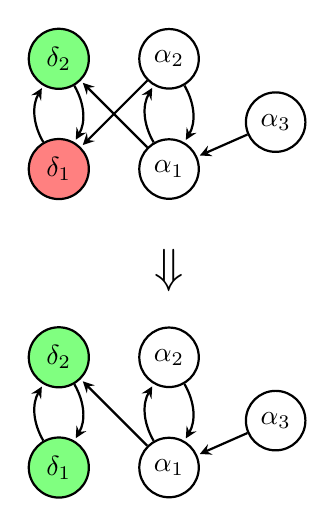
\begin{tikzpicture}[->,>=stealth,shorten >=1pt,auto,node distance=1.4cm, thick,main node/.style={circle,draw,font=\bfseries},uncertain/.style={rectangle,draw,dashed,font=\bfseries}]
    \node[main node,fill=red!50] (delta1) {$\delta_1$};
    \node[main node,fill=green!50] (delta2) [above of=delta1] {$\delta_2$};
    \node[main node] (alpha1) [right of=delta1] {$\alpha_1$};
    \node[main node] (alpha2) [right of=delta2] {$\alpha_2$};
    \node[main node] (alpha3) [below right=0.25cm and 0.8cm of alpha2] {$\alpha_3$};

    \path[->] (delta1) edge[bend left] (delta2)
        (delta2) edge[bend left] (delta1)
        (alpha2) edge (delta1)
        (alpha1) edge (delta2)
        (alpha3) edge (alpha1)
        (alpha1) edge[bend left] (alpha2)
        (alpha2) edge[bend left] (alpha1);

    \node[below=0.5cm of alpha1] {\LARGE$\Downarrow$};

    \node[main node,fill=green!50,below=3cm of delta1] (ddelta1) {$\delta_1$};
    \node[main node,fill=green!50] (ddelta2) [above of=ddelta1] {$\delta_2$};
    \node[main node] (aalpha1) [right of=ddelta1] {$\alpha_1$};
    \node[main node] (aalpha2) [right of=ddelta2] {$\alpha_2$};
    \node[main node] (aalpha3) [below right=0.25cm and 0.8cm of aalpha2] {$\alpha_3$};

    \path[->] (ddelta1) edge[bend left] (ddelta2)
        (ddelta2) edge[bend left] (ddelta1)
        (aalpha1) edge (ddelta2)
        (aalpha3) edge (aalpha1)
        (aalpha1) edge[bend left] (aalpha2)
        (aalpha2) edge[bend left] (aalpha1);

\end{tikzpicture}

  \end{column}

\end{columns}

\vfill

\begin{center}
  \large
  \textbf{Can we minimize semantic and syntactic change simultaneously?}
\end{center}

\end{frame}


% ------------------------------------------------------------------
% Slide 2 -- Formula-based enforcement
% ------------------------------------------------------------------
\begin{frame}{Formula-based enforcement}

\begin{center}
  A formula-based enforcement instance specifies \textbf{propositional constraints}
  which should be satisfied by the resulting argumentation framework.
\end{center}

\vspace{0.4em}

\begin{columns}[T,onlytextwidth]

  \begin{column}{0.31\textwidth}
    \begin{block}{$\Phi^{+}$: desired behavior}
      Formulas that should hold in
      \textbf{some extension}.

      \vspace{0.4em}

      \[
        in_{a} \land in_{b}
      \]
    \end{block}
  \end{column}

  \begin{column}{0.31\textwidth}
    \begin{block}{$\Phi^{-}$: forbidden behavior}
      Formulas that should hold in
      \textbf{no extension}.

      \vspace{0.4em}

      \[
        \neg in_{b} \lor \neg in_{c}
      \]
    \end{block}
  \end{column}

  \begin{column}{0.31\textwidth}
    \begin{block}{$\Phi^{R}$: structural constraints}
      Formulas constraining the
      \textbf{attack relation}.

      \vspace{0.4em}

      \[
        att_{a,b} \rightarrow att_{b,c}
      \]
    \end{block}
  \end{column}

\end{columns}

\vspace{0.7em}

\begin{block}{Hard and soft constraints}
Weights on formulas distinguish requirements that \textbf{must} be satisfied from
\textbf{preferences}.
\end{block}

\begin{center}
  \textbf{Constraints on semantic and syntactic change can be combined into a single instance.}
\end{center}

\end{frame}


% ------------------------------------------------------------------
% Slide 3 -- Generality / novelty
% ------------------------------------------------------------------
\begin{frame}{Generality of formula-based enforcement}

  Formula-based enforcement captures various existing enforcement notions as special cases:
  \begin{itemize}
    \item extension enforcement \mjcite{BaumannB10,Coste-MarquisKM15,WallnerNJ17}
    \item status enforcement \mjcite{NiskanenWJ16}
    \item rejection enforcement \mjcite{Heine024}
    \item argumentation framework synthesis \mjcite{synthesis19}
  \end{itemize}

    \begin{exampleblock}{New enforcement variants}
      For example:
      \[
        in_a \xmapsto{w} \infty, \qquad in_b \xmapsto{w} \infty, \qquad
        in_a \land in_b \xmapsto{w} k > |A|^2
      \]
      Require $a$ and $b$ to be individually accepted, while
      \textbf{preferably accepting them together}.
    \end{exampleblock}

\end{frame}


% ------------------------------------------------------------------
% Slide 4 -- Complexity
% ------------------------------------------------------------------
\begin{frame}{Complexity of formula-based enforcement}

Expressivity of formula-based enforcement comes at a price:
high computational complexity.

\medskip

\begin{center}
  \large
  \begin{tabular}{lc}
    \toprule
    \textbf{Semantics} & \textbf{Complexity} \\
    \midrule
    Grounded    & $\NP$-complete \\ \hline\hline
    Admissible  & $\Sigma_2^p$-complete \\
    Complete    & $\Sigma_2^p$-complete \\
    Stable      & $\Sigma_2^p$-complete \\ \hline\hline
    Preferred   & $\Sigma_3^p$-complete \\
    \bottomrule
  \end{tabular}
\end{center}

\vspace{0.8em}

\begin{center}
  \large
  \textbf{Can we still solve practical instances exactly?}
\end{center}

\end{frame}


% ------------------------------------------------------------------
% Slide 5 -- Algorithm
% ------------------------------------------------------------------
\begin{frame}{MaxSAT-based counterexample-guided abstraction refinement (CEGAR)}

\textbf{Exact algorithm for $\Sigma_2^p$-complete variants:}
instead of encoding the full problem at once,
iteratively solve an easier abstraction
and refine it when counterexamples are encountered.

\bigskip

\begin{columns}[T,onlytextwidth]

  \begin{column}{0.55\textwidth}

  \centering

  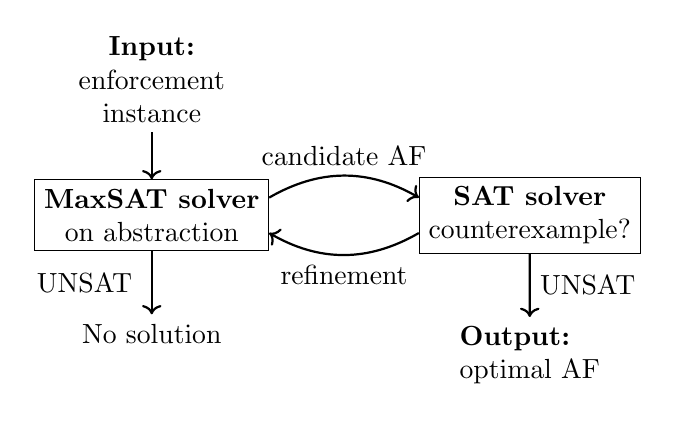
\begin{tikzpicture}[scale=0.8]
  \node [align=center, draw] at (0,0) (RMP) {\textbf{MaxSAT solver} \\ on abstraction};
  \node [align=center, draw] at (6,0) (PP) {\textbf{SAT solver} \\ counterexample?};
  \node [align=center, above=0.6 of RMP]  (I) { \textbf{Input:} \\ enforcement\\instance};
  \draw [->, thick] (I.south) to (RMP.north);
  \draw[->, thick] ([yshift=8pt] RMP.east) to[bend left] node[above,align=center] {candidate AF} ([yshift=8pt] PP.west);
  \draw[->, thick] ([yshift=-8pt] PP.west) to[bend left] node[above,align=center] {} node[below,align=center] {refinement} ([yshift=-8pt] RMP.east);
  \node [align=left, below=0.8 of PP] (O) {\textbf{Output:} \\ optimal AF};
  \node [align=left, below=0.8 of RMP] (X) {No solution};
  \draw [->, thick] (PP.south) to node[right,align=center] { UNSAT } (O.north);
  \draw [->, thick] (RMP.south) to node[left,align=center] { UNSAT } (X.north);
\end{tikzpicture}

  \end{column}

  \begin{column}{0.42\textwidth}

    \textbf{High-level idea}

    \begin{enumerate}
      \item Call a MaxSAT solver to find an optimal candidate attack structure.
      \item Check using a SAT solver whether the candidate AF has a counterexample extension.
      \item If a counterexample exists,
            refine the abstraction by adding a clause which excludes it.
      \item Repeat until no counterexample remains.
    \end{enumerate}

  \end{column}

\end{columns}

\end{frame}


% ------------------------------------------------------------------
% Slide 6 -- Experimental results
% ------------------------------------------------------------------
\begin{frame}{How far can the algorithm scale?}

\begin{columns}[T,onlytextwidth]

  \begin{column}{0.6\textwidth}

    \centering

    \myfigure[0.7\columnwidth]{solving_time_vs_arguments.pdf}

  \end{column}

  \begin{column}{0.4\textwidth}

    \vspace{10pt}

    \textbf{Setup}

    \begin{itemize}
      \item 950 generated instances.
      \item $n = 20,40,\ldots,200$ arguments.
      \item Admissible vs. stable semantics.
      \item 600 s timeout per instance.
    \end{itemize}

    \vspace{0.3em}

    \textbf{Observations}

    \begin{itemize}
      \item Stable semantics scales to roughly
            70 arguments.
      \item Admissible semantics requires far more CEGAR iterations: \\
            $\approx$ 2100 vs. $\approx$ 46.
    \end{itemize}

  \end{column}

\end{columns}

\vfill

\begin{center}
  \url{https://bitbucket.org/andreasniskanen/phiaf}
\end{center}

\end{frame}


% ------------------------------------------------------------------
% Slide 7 -- Takeaways
% ------------------------------------------------------------------
\begin{frame}{Summary}

\begin{block}{Contributions}
\textbf{Formula-based enforcement:} unified language for expressing semantic and syntactic constraints
for enforcement in abstract argumentation via weighted propositional formulas.
\begin{itemize}
  \item \textbf{Generalizes} various existing notions while enabling new forms of enforcement.
  \item \textbf{Complexity} ranges from NP-completeness to $\Sigma_3^{p}$-completeness.
  \item \textbf{Exact algorithm} for $\Sigma_2^p$-complete variants by employing MaxSAT-based CEGAR.
  \item \textbf{Empirical evaluation} demonstrates scalability to moderately-sized AFs.
\end{itemize}
\end{block}

\vspace{1em}

\begin{center}
  \large Thank you for your attention! Questions?
\end{center}

\end{frame}


% ------------------------------------------------------------------
% Optional backup slides
% ------------------------------------------------------------------
\appendix

\backupbegin
\begin{frame}{Bibliography}
\normalsize
\def\newblock{\hskip .11em plus .33em minus .07em} % important line
\bibliographystyle{apacite}
\bibliography{ijcai26}
\end{frame}
\backupend

\end{document}
